\chapter{OpenHAB}

After analyzing the main products and services in the field of home automation and voice assistance, I must choose the solution
that can best fit this project. One of its requirements is to use as many open source and free technologies as possible, and that
the final product is easily usable by the final user and sufficiently flexible to adapt it to our needs.

OpenHAB is fully open source and completely free, and has reached a level of maturity where it is highly stable and intuitive. In its
most recent version, it provides an user interface that automatize many tasks that a standard user might not know how to do. And,
of course, it can integrate many devices from different vendors, as In have mentioned in the previous chapters, which is also one of
the most important matters for reaching our objective.

In this chapter, I will explore in depth this home automation platform and all its possibilities, in order to have a better general idea
about it when building the final system.

\section{Introduction}
As I mentioned in previous chapters, openHAB (open Home Automation Bus) is a completely free, technology agnostic and open
source platform for home automation. 

OpenHAB software is capable of integrating different domotic systems, devices and technologies into a single solution. It also
provides uniform user interfaces, and a common approach to automation rules across the entire system, regardless of the number
of manufacturers and sub-systems involved.\cite{openHABDocs}

The platform runs on many popular platforms including Linux, Windows and macOS. It is also popular to install it in systems like the
Raspberry Pi, and openHAB even provides a special distribution for this computer, called \textit{openHABian}, a simplified way of
getting up and running openHAB, but offering the complete experience.

OpenHAB defines also a community of users, contributors and maintainers, working together on the improvement of the system.
Everything related to the community is in the openHAB community forum. The community is very active and helpful, and thanks
to them I have always found a way to solve my issues.

\bigskip
\section{History of openHAB}
The history of openHAB begins in 2010, when Kai Kreuzer, a smart home enthusiast from Germany, developed in Java and using the
OSGi technology (Open Services Gateway Initiative) as the basis, which is a set of specifications that define a dynamic component 
system for Java. The use of this technology makes it easier to update the services independently and their implementation. It favor
the expandability of the system.

In 2013, openHAB becomes an official Eclipse project under the name of Eclipse SmartHome, but they decide to keep both projects
active and to develop them at the same time. In Eclipse SmartHome would maintain the architecture and the functionalities from the
previous openHAB, and in openHAB they would study how to integrate the different devices and technologies that it supports via 
add-ons.

The newest version, OpenHAB 2, has been the biggest change that OpenHAB has suffered since its initial launch. It includes more 
add-ons and some changes that simplify much more the process for developers, as well as implementing Apache Karaf underneath, 
which greatly extends its possibilities. In addition, the UIs have been improved, improving greatly the user experience. OpenHAB 2 is
much easier to install, and it automates many repetitive processes that might result hard for some users.

\bigskip
\section{Structure}
OpenHAB works thanks to add-ons, which can extend its capabilities to fit each user’s needs, from User Interfaces, to the ability to 
interact with a large and growing number of physical \textit{Things}. Add-ons may come from the OpenHAB 2 distribution, the Eclipse
SmartHome project Extensions, or from the OpenHAB 1 distribution.

\begin{figure}
	\centering
	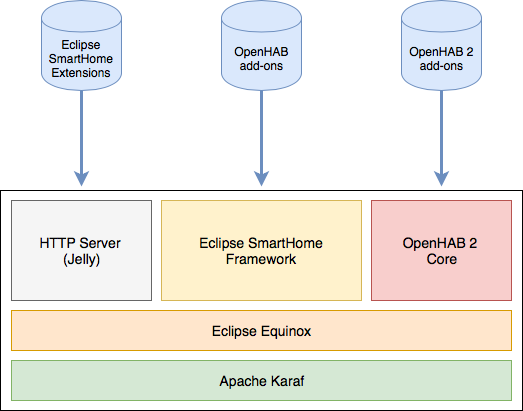
\includegraphics[width=0.9\textwidth]{images/Chapter_05/openhab-architecture.png}
	\caption{OpenHAB architecture}
	\label{fig:openhab-architecture}
\end{figure}

The figure \ref{fig:openhab-architecture} shows the overall architecture of openHAB 2. In the lowest layer, we can find Apache Karaf.
Apache Karaf is basically a modular and open source OSGi runtime environment that can host any kind of applications.\cite{apacheKaraf}
 
Next, there is Eclipse Equinox, which is also an implementation of the OSGi core framework specification. But the goal of the Equinox
project is to be a first class OSGi community and foster the vision of Eclipse as a landscape of bundles too. Equinox is responsible for
developing and delivering the OSGi framework implementation used for all of Eclipse.\cite{eclipseEquinox} 

The next and last level is divided in three parts. The first one is the Jetty HTTP server, also part of Eclipse, which provides a Web server 
and javax.servlet container, plus support for HTTP/2, WebSocket, OSGi, JMX, JNDI and JAAS, among others.\cite{eclipseJetty} Secondly,
we can find the Eclipse SmartHome Framework , the framework to build end user solutions on top like openHAB, that I mentioned 
before.\cite{eclipseSmartHomeDocs} The last part is the core of openHAB 2, which provides the full solution.

As the diagram in the figure \ref{fig:openhab-architecture} indicates, we can add to this system extensions from Eclipse SmartHome and
add-ons from the first and second version of openHAB.

\bigskip
\section{Concepts}
As Eclipse SmartHome is the logic part of OpenHAB 2, all the elements I am listing are part of it. Eclipse SmartHome strictly differentiates
between the physical view and the functional view of the system. The physical view is more familiar to us, and focuses on the devices
on the system, the connections between them (e.g. wires, Netatmo devices, WiFi hardware) and other physical aspects of the system.
The functional view focuses on how information about the devices, connections, and so on, is represented in user interfaces, focusing
on how rules effect representations of physical devices in software. The functional view focuses on how an action in a user interface
affects the software associated with the physical device it represents.

That said, I will explore the different elements that Eclipse SmartHome considers in this section. The greatest difference that we can find
related to devices, is between \textit{Things} and \textit{Items}. Generally speaking, Things represent physical systems that can be added
to openHAB and Items represent functionalities that can be used by the applications. The figure \ref{fig:openhab-concepts-basics} 
shows a graphical explanation of this concept, though I will explain in depth these concepts below.

\begin{figure}
	\centering
	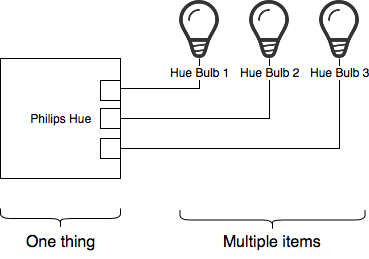
\includegraphics[width=0.6\textwidth]{images/Chapter_05/openhab-concepts-basics.png}
	\caption{A simplification of the concepts of Thing and Item}
	\label{fig:openhab-concepts-basics}
\end{figure}

\subsection{Things}
Things are the entities that can physically be added to a system and which can potentially provide many functionalities in one. They do
not need to be devices, but they can also represent a web service, or any other manageable source of information and functionality.
Things are important in the setup and configuration process, when the user has to add his devices to the system, but they are not for
the operation, when everything is up and running.

Things can have configuration properties, which can be optional or mandatory. Such properties can be basic information like an IP address,
an access token for a web service or a device specific configuration that alters its behavior.

\subsubsection{Channels}
Channels are part of the Things, and they represent the different functions they provide. Where the Thing is the physical entity 
or source of information, the Channel is a concrete function from this Thing. For example, some Philips Hue light bulbs have a color 
temperature Channel and a color Channel, both providing functionality of the one light bulb Thing to the system. For sources of
information the Thing might be the local weather with information from a web service with different Channels like temperature, pressure 
and humidity.

Channels are linked to Items, where such links are the glue between the virtual and the physical layer. Once such a link is established,
a Thing reacts on events sent for an item that is linked to one of its Channels. Likewise, it actively sends out events for Items linked to its 
Channels

\subsubsection{Bridges}
Bridges are special types of Things. They are \textit{Things} that need to be added to the system in order to gain access to other Things.
For example, an IP gateway for some non-IP based home automation system or a web service configuration with authentication information
which every Thing from this web service might need.

Some Bindings come with a Bridge, like the \textit{PHC Binding}, which allows to integrate modules of PHC in openHAB.\cite{openHABPHCBinding}

\subsubsection{Thing Status}
Every Thing has a status, which helps to identify possible problems with the device or service and gives useful information to the user
in any moment. The statuses are limited to seven types, as the table \ref{table:thing-statuses} shows.

\begin{table}[]
	\begin{center}
		\resizebox{\textwidth}{!}{
		\begin{tabular}{|c|p{0.8\linewidth}|}
			\hline
			\textbf{Status} & \multicolumn{1}{c|}{\textbf{Description}}                                                                                                                                                                                                                                                                                                                                                                                                                                                 \\ \hline
			UNINITIALIZED & This is the initial status of a Thing, when it is added or the framework is being started. This status is also assigned, if
			the initializing process failed or the binding is not available. Commands, which are sent to Channels will not be processed. \\ \hline
			INITIALIZING & This state is assigned while the binding initializes the Thing. It depends on the binding how long the initializing process 
			takes. Commands, which are sent to Channels will not be processed. \\ \hline
			UNKNOWN & The handler is fully initialized but due to the nature of the represented device/service it cannot really tell yet whether the
			Thing is ONLINE or OFFLINE. Therefore the Thing potentially might be working correctly already and may or may not process commands. 
			But the framework is allowed to send commands, because some radio-based devices may go ONLINE if a command is sent to them. The 
			handler should take care to switch the Thing to ONLINE or OFFLINE as soon as possible. \\ \hline
			ONLINE & The device/service represented by a Thing is assumed to be working correctly and can process commands. \\ \hline
			OFFLINE & The device/service represented by a Thing is assumed to be not working correctly and may not process commands. But the 
			framework is allowed to send commands, because some radio-based devices may go back to ONLINE, if a command is sent to them. \\ \hline
			REMOVING & The device/service represented by a Thing should be removed, but the binding did not confirm the deletion yet. Some 
			bindings need to communicate with the device to unpair it from the system. Thing is probably not working and commands can not be 
			processed. \\ \hline
			REMOVED & This status indicates that the device/service represented by a Thing was removed from the external system after the 
			REMOVING was initiated by the framework. Usually this status is an intermediate status because the Thing gets removed from the 
			database after this status was assigned. \\ \hline
		\end{tabular}}
	\caption{The statuses of Things in openHAB 2}
	\label{table:thing-statuses}
	\end{center}
\end{table}

The statuses UNINITIALIZED, INITIALIZING and REMOVING are set by the framework, where as the statuses UNKNOWN, ONLINE and OFFLINE
are assigned from a binding. Additionally, the REMOVED state is set by the binding to indicate that the removal process has been completed,
that it, the Thing must have been in REMOVING state before.

\subsubsection{Status Transitions}
The figure \ref{fig:status-transitions} shows the possible status transitions in openHAB.

\begin{figure}
	\centering
	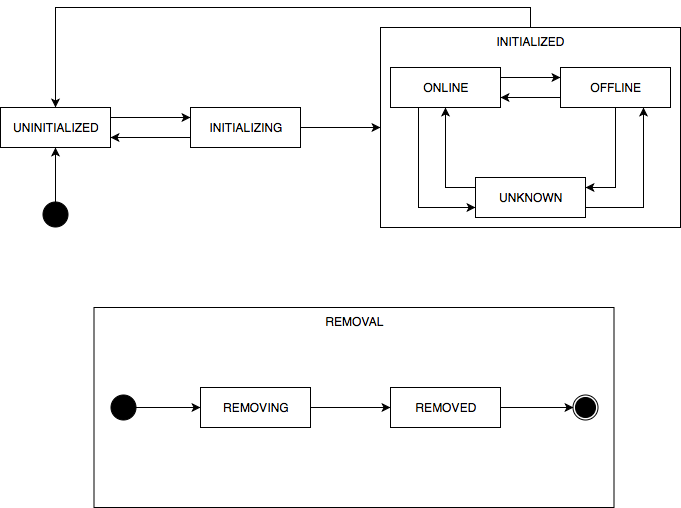
\includegraphics[width=1\textwidth]{images/Chapter_05/status-transtitions.png}
	\caption{Thing status transitions}
	\label{fig:status-transitions}
\end{figure}

The initial state of a Thing is UNINITIALIZED. From UNINITIALIZED the Thing goes into INITIALIZING. If the initialization fails, the 
Thing goes back to UNINITIALIZED. If the initialization succeeds, the binding sets the status of the Thing to UNKNOWN, ONLINE
or OFFLINE, which all mean that the Thing handler is fully initialized. From one of this states the Thing can go back into UNINITIALIZED,
REMOVING or REMOVED. The statuses REMOVING and REMOVED can also be reached from any of the other states.

\subsection{Items}
Eclipse SmartHome has a strict separation between the physical world (Things) and the application, which is built around the concept
of \textit{Items} (also known as the \textit{virtual layer}).

As mentioned at the beginning of this section, Items represent functionalities that can be used by the applications, mainly user 
interfaces or automation logic. Items also have a state and are used through events.

Each openHAB Item must be between the list of types that the table \ref{table:openhab-item-types} specifies.

\begin{table}[]
	\centering
	\resizebox{\textwidth}{!}{%
		\begin{tabular}{|l|l|l|}
			\hline
			\multicolumn{1}{|c|}{\textbf{Color}}                          & \multicolumn{1}{c|}{\textbf{Description}}                                                                          & \multicolumn{1}{c|}{\textbf{Command Types}}                                           \\ \hline
			Color                                                         & Color information (RGB)                                                                                            & \begin{tabular}[c]{@{}l@{}}OnOff, IncreaseDecrease,\\ Percent, HSB\end{tabular}       \\ \hline
			Contact                                                       & \begin{tabular}[c]{@{}l@{}}Item storing status of e.g. door/window \\ contacts\end{tabular}                        & OpenClose                                                                             \\ \hline
			DateTime                                                      & Stores date and time                                                                                               &                                                                                       \\ \hline
			Dimmer                                                        & \begin{tabular}[c]{@{}l@{}}Item carrying a percentage value for \\ dimmers\end{tabular}                            & \begin{tabular}[c]{@{}l@{}}OnOff, IncreaseDecrease,\\ Percent\end{tabular}            \\ \hline
			Group                                                         & \begin{tabular}[c]{@{}l@{}}Item to nest other Items / collect them \\ in Groups\end{tabular}                       &                                                                                       \\ \hline
			Image                                                         & Holds the binary data of an image                                                                                  &                                                                                       \\ \hline
			Location                                                      & Stores GPS coordinates                                                                                             & Point                                                                                 \\ \hline
			Number                                                        & \begin{tabular}[c]{@{}l@{}}Stores values in number format, takes \\ an optional dimension suffix\end{tabular}      & Decimal                                                                               \\ \hline
			\begin{tabular}[c]{@{}l@{}}Number:\\ <dimension>\end{tabular} & \begin{tabular}[c]{@{}l@{}}Like Number, but with additional \\ dimension information for unit support\end{tabular} & Quantity                                                                              \\ \hline
			Player                                                        & \begin{tabular}[c]{@{}l@{}}Allows to control players (e.g. \\ audio players)\end{tabular}                          & \begin{tabular}[c]{@{}l@{}}PlayPause, NextPrevious, \\ RewindFastforward\end{tabular} \\ \hline
			Rollershutter                                                 & Typically used for blinds                                                                                          & \begin{tabular}[c]{@{}l@{}}UpDown, StopMove, \\ Percent\end{tabular}                  \\ \hline
			String                                                        & Stores texts                                                                                                       & String                                                                                \\ \hline
			Switch                                                        & Typically used for lights                                                                                          & OnOff                                                                                 \\ \hline
		\end{tabular}%
	}
	\caption{Types of Items in openHAB 2}
	\label{table:openhab-item-types}
\end{table}

\subsubsection{Group Items}
Group Items are a special kind of items that collect other Items into Groups. Group Items can themselves be members of other Group Items.
Depending on the user interface, it might display Group Items as single entries and provide navigation to its members.

With Group Items, it is also possible to derive their state from their member items. To derive a state the Group Item must be constructed using
a base Item and a Group function. Between the available Group functions we can find common operators such as EQUALITY, AND, OR, NAND,
NOR, SUM, AVG, MIN and MAX, among others.

\subsubsection{Links}
Links are the glue between Things and Items. They are associations between exactly one Thing Channel and one Item. If a Channel is 
linked to an Item, it is enabled, which means that the functionality that the Item represents is handled through the given Channel. 
Channels can be linked to multiple Items and Items can be linked to multiple Channels.

\subsection{Thing Discovery}
Thing Discovery is the process that the system makes in order to show the devices connected in your network. Many technologies, 
devices and systems can be discovered automatically or browsed through an API.

In Eclipse SmartHome bindings implement \textit{Discovery Services} for things, which provide \textit{Discovery Results}. All Discovery 
Results are regarded as suggestions to the user and are put into the \textit{Inbox}.

\subsubsection{Inbox}
he inbox holds a list of all discovered things from all active discovery services. A discovery result represents a discovered thing of a 
specific thing type, that could be instantiated as a thing. The result usually contains properties that identify the discovered things 
further like IP address or a serial number. Each discovery result also has a timestamp when it was added to or updated in the inbox 
and it may also contain a time to live, indicating the time after which it is be automatically removed from the inbox.

Discovery results can either be ignored or approved, where in the latter case a thing is created for them and they become available in 
the application. If an entry is ignored, it will be hidden in the inbox without creating a thing for it.

There are options for automating the approval or ignorance of devices.




